\chapter{Sequential circuits}
Sequential logic circuits are such that the outputs depends not only on the present value of the input but also on theyr previous values.
To achive this goal we need gates that have to remember the history of the input data; such circuits are said to have a state.\\
There are 2 basic memory elements: latches and flip-flops.\\
	
\vspace{5mm}

Latches are tipically used to build flip-flops in the master-slave configuration (that is the most adopted memory element). Both latches and flip-flop are in theyr basic configuration a 3 port devices with 2 inputs an 1 output: the two inputs are D data in and CLK clock , the output is Q (and an eventual $\bar{Q}$).\\
\vspace{5mm}
\centering
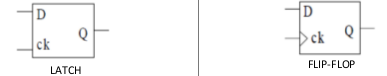
\includegraphics[width=0.5\textwidth]{C10_1.png}\\
\raggedright
\vspace{7mm}

A latch is a memory element sensitive to the level of the clock, while the flip-flop is sensitive to the edge of the clock signal. We will refer to a latch as to an element level-triggered, and to the flip-flop as an element edge triggered.\\

\vspace{5mm}
\centering
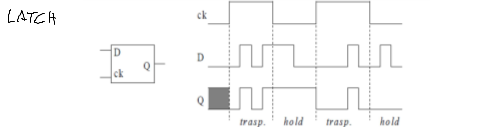
\includegraphics[width=0.7\textwidth]{C10_2.png}\\
\raggedright

\centering
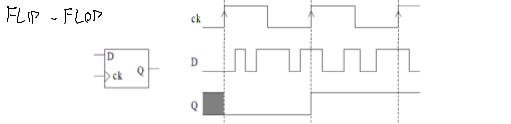
\includegraphics[width=0.7\textwidth]{C10_3.png}\\
\raggedright
\vspace{5mm}

To build up a flip-flop we can use the master-slave structure using 2 latches one positive and one negative connected as shown in figure

\vspace{5mm}
\centering
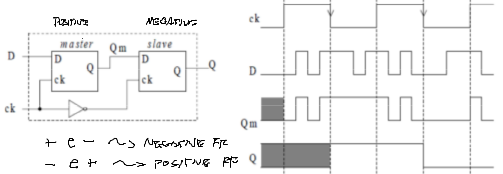
\includegraphics[width=0.8\textwidth]{C10_4.png}\\
\raggedright
\vspace{5mm}

The main applications for this structrures are four: data sotrage in foreground memory (RAM is a background element), frequency divider, counters and finite state machines (FSM)





\section{Finite state machines (FSM)}

\centering
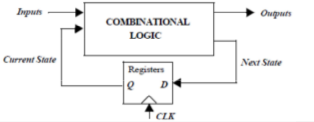
\includegraphics[width=0.5\textwidth]{C10_5.png}\\
\raggedright

It’s a compound of a logic circuit and one or more flip-flops adopted as memory elements to store data.\\
\vspace{3mm}
There are some importants times that has to be considered when we deal with memory elements
\begin{itemize}

\item The set-up time $t_{su}$ is the time that the input data must be valid before the sensitive edge of the clock.

\item The hold time $t_{hold}$ is the time that the input data must remain stable after the edge of the clock (it can be also negative).

\item If the previous times are verified the input data is copied at the output after a time $t_{cq}$ that is form the edge of the clock to the cross of half supply at the output.

\end{itemize}

For a generic FSM we can underline two time constraints that have to be respected for the circuit to work.\\

\centering
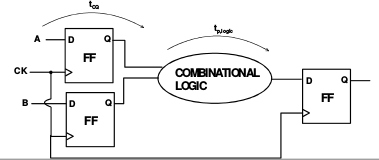
\includegraphics[width=0.5\textwidth]{C10_6.png}\\
\raggedright

\subsection{Max-delay constraint}
Denoting T as the clock period and $t_{p,logic}^{max}$ as the maximum delay of the logic, we have to ensure that 
\begin{equation}
t_{cq}+t_{su}+ t_{p,logic}^{max} \le T
\end{equation}
That can be translated in 
\begin{equation}
t_{p,logic}^{max}\le T-(t_{cq}+t_{su})=T-t_{overhead}
\end{equation}
The signal has to pass throught the flip-flop and the logic and be present at the input od the memory element a set-up time before the edge of the clock.\\

\subsection{Min-delay constraint}
The hold constraint says that the signal cannot propagate throught the flip-flop and the logic too fast or it will remain at the input of the flip-flop for too little time
\begin{equation}
t_{cq}+ t_{p,logic}^{min} \ge t_{hold}
\end{equation}


\section{Static memory devices}

Typical static memory device is a couple of inverter connected in positive loop one another. This type of structure gives us (overlapping the 2 characteristics) has only 2 stable ponis (ground or $V_{DD}$) and one metastable point as shown in figure

\centering
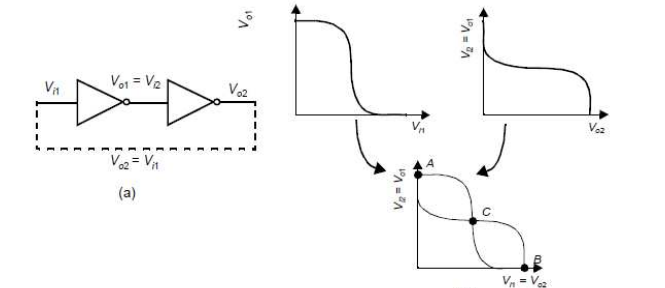
\includegraphics[width=0.7\textwidth]{C10_7.png}\\
\raggedright

\subsection{Multiplexer-based static latch}

\centering
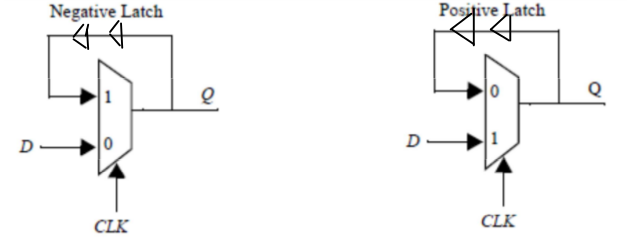
\includegraphics[width=0.5\textwidth]{C10_8.png}\\
\raggedright

The loop can be opened to write the data or closed to store it. The mux is implemented with transimssion gates as in figure (positive latch in figure)

\centering
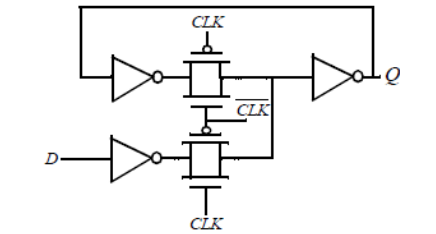
\includegraphics[width=0.35\textwidth]{C10_9.png}\\
\raggedright

Since when implementing a clocked element the number of transistors connected to the clock signal play a foundamental role in power dissipation (since theyr $\alpha_{sw}=1$) we can also use this structure

\centering
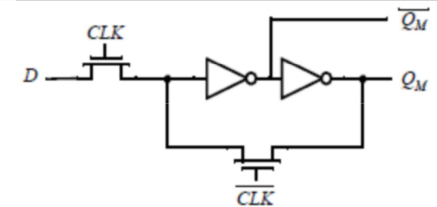
\includegraphics[width=0.35\textwidth]{C10_10.png}\\
\raggedright

This structure has of course some drawbacks; the nmos passes a degraded high voltage that implies a larger propagation delay, reduced noise margins and static power consumptions of the inverters.\\


\subsection{Multiplexer-based static flip-flop}

The multiplexer-based static flip-flop is implemented in the master-slave configuration as follows

\centering
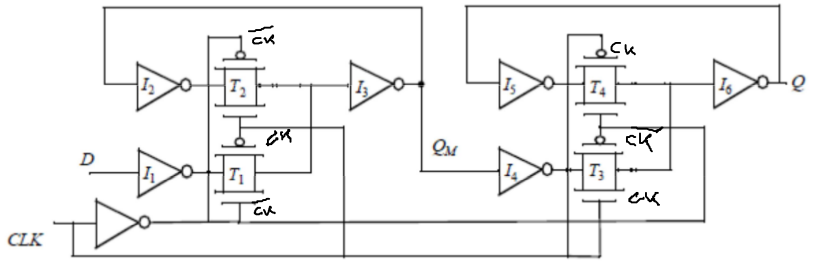
\includegraphics[width=0.7\textwidth]{C10_11.png}\\
\raggedright

We define $t_{inv}$ as the propagation delay of the inverter and $t_{tx}$ as the propagation delay of a trasmission gate; doing so we can hilight the different time constraint of this device.\\

\begin{itemize}

\item 
{\bf Set-up time}\\
We need that the input signal passes throught the first inverter $I_1$ the trasmission gate $T_1$ and the other 2 inverters $I_2,I_3$ otherwise there is the possibility to have conflicts or incorrect values on the 2,3 inverters so
\begin{equation}
t_{su}=3t_{inv}+t_{tx}
\end{equation}

\item 
{\bf Propagation delay}\\
Due to set-up time we already have the signal after the $I_4$ inverter. The signal have to be propagated throught the trasmission gate $I_4$ and the inverter $I_6$
\begin{equation}
t_{cq}=t_{inv}+t_{tx}
\end{equation}

\item
{\bf Hold time}\\
The rising edge of the clock turns the transmission gate $T_1$ off, thus any change of the input signal does not cause a change of the flip-flop state.
Since the inverter $I_1$ has a propagation delay, the input D can change also before the rising edge of the clock without being sampled by the transmission gate; the hold time is negative
\begin{equation}
t_{hold}=-t_{inv}
\end{equation}

\end{itemize}


\subsection{Time constraints rigorous definitions}

%TO DO%




\subsection{Brute force filp-flop}

To reduce the number of transistors involved in a flip-flop (and also the problem of high number of transistor feeded by the clock signal) we can use a ratioed solution like the brute-force flip-flop

\centering
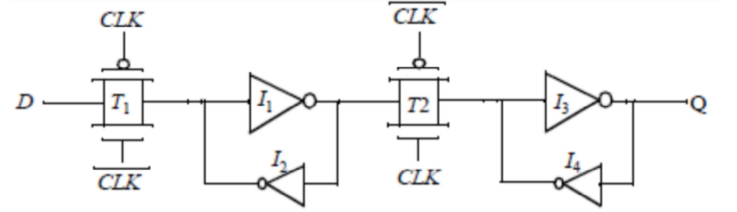
\includegraphics[width=0.7\textwidth]{C10_12.png}\\
\raggedright

The first latch can be written only if the first trasmission gate and the driver circuit are stroger than the feedback inverter to change the state at the input of $I_1$.\\
Moreover there is a problem of "reverse conduction". When the clock is high the second trasmission gate is closed and there can be a conflict between the first and the second stage; $I_4$ has to be sized in a way that can't overwhelm $I_1$ (if this happen the first loop can change it's state).\\

\subsection{Clock overlap}

Due to different paths the clk and the $\bar{clk}$ signals aren't sincronized but they have a period of overlap (0-0 or 1-1 overalap) that can cause wrong toggles (due to critical races that is that the output is connected to the input in 1-1 overlap) or undefined states (due to 0-0 overlap).\\
\vspace{5mm}
A solution to solve the 1-1 overlap is the adoption of the following circuit to generate the 2 clock signals

\centering
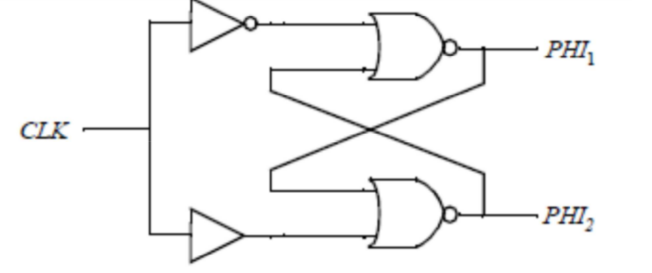
\includegraphics[width=0.5\textwidth]{C10_13.png}\\
\raggedright

\centering
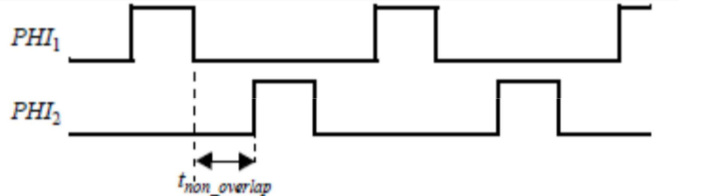
\includegraphics[width=0.5\textwidth]{C10_14.png}\\
\raggedright

There is never a period when both signals are high but on the other hand there are a lot of 0-0 overlaps that can destroy the state if this condition last for too long.\\

\section{Dynamic memory devices}
This memory elements store the data as chage across a capacitance as the dynamics gates. The main drawback is that charge may be lost if the data is not refreshed for a long time.\\
The classical master-slave implementation of a flip-flop reduces to 8 transistors as shown in figure (the capacitance are the parasitic of the trasmission gate and of the inverter)

\vspace{2mm}
\centering
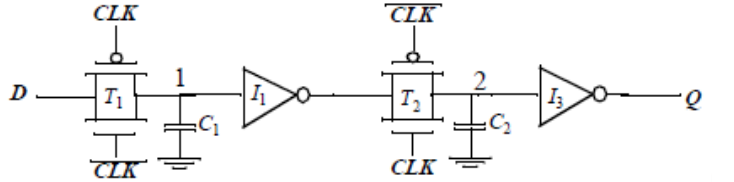
\includegraphics[width=0.7\textwidth]{C10_15.png}\\
\raggedright
\vspace{2mm}

The sensitive times related to this implementation are
\begin{itemize}
\item 
{\bf Set-up time}\\
The time needed to the trasmission gate to pass the data to the node "1"
\begin{equation}
t_{su}=t_{tx}
\end{equation}

\item 
{\bf Propagation delay}\\
Is the time that the data use to pass form the node "1" to the output (the transition throught the inverter has not yet passed)
\begin{equation}
t_{cq}=t_{inv}+2t_{tx}
\end{equation}

\item
{\bf Hold time}\\
The hold time is 0

\end{itemize}
\vspace{5mm}
During both clock overlaps in this gate we get a direct connection between in and out.\\
The 0-0 overlap can be avoided making the overlap period small enough that the signal does not reach the output 
\begin{equation}
t_{overlap-00}\le t_{inv}+2t_{tx}
\end{equation} 
The 1-1 overlap can be avoided establishing a hold time large enough 
\begin{equation}
t_{overlap-11}\le t_{hold}
\end{equation}

\subsection{$C^2 MOS$}
This is a dynamic solution insensitive to clock overlap problems. $C^2$ stand for clocked cmos and the implementation is shown in figure 

\centering
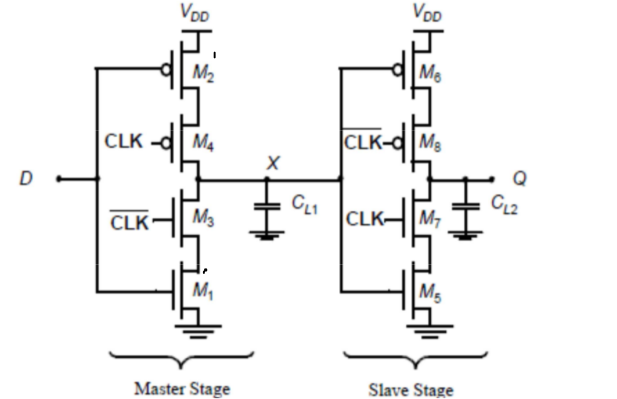
\includegraphics[width=0.5\textwidth]{C10_16.png}\\
\raggedright

The two latches are tristate inverters : the output node can be high low or at high impedance state depending on the inputs. The figure represents a positive edge triggered ff.\\
The only problem that arise is just after a 1-1 overlap as soon as $\bar{clk}$ transit back to 0 the Q node is turned up to $V_{DD}$. This can be solved only imposing a hold time constraint.\\


\subsection{True single phase clock TSPC flip-flops}
This implementation avoid the clock overlap problem by using only the clok signal avoiding it's complement relying on the fact that pmos and nmos are on for different voltages.

\centering
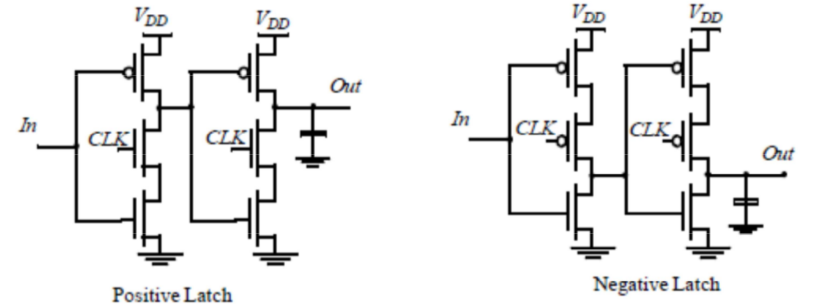
\includegraphics[width=0.5\textwidth]{C10_17.png}\\
\raggedright

When clk is high the circuit is a cascade of two inverters and when the clock is low it's an open circuit in the positive latch and vice versa for the negative so that no direct path can be formed.\\
\vspace{5mm}


To spare transistors we can use the so called "split out" scheme 

\centering
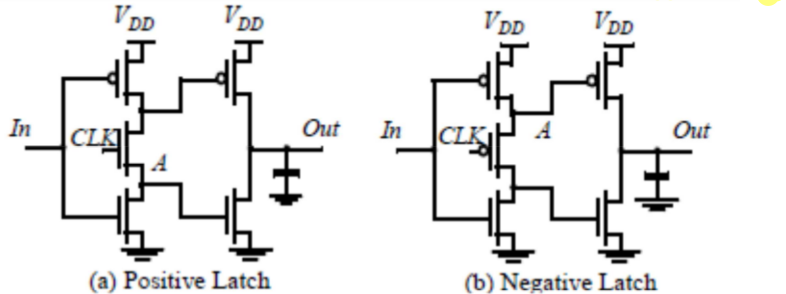
\includegraphics[width=0.5\textwidth]{C10_18.png}\\
\raggedright

The drawback in this case is that the node A cannot feature a full swing leading to worst performance in terms of propagation delay.\\



\section{Scheme of all flip-flops implementations}
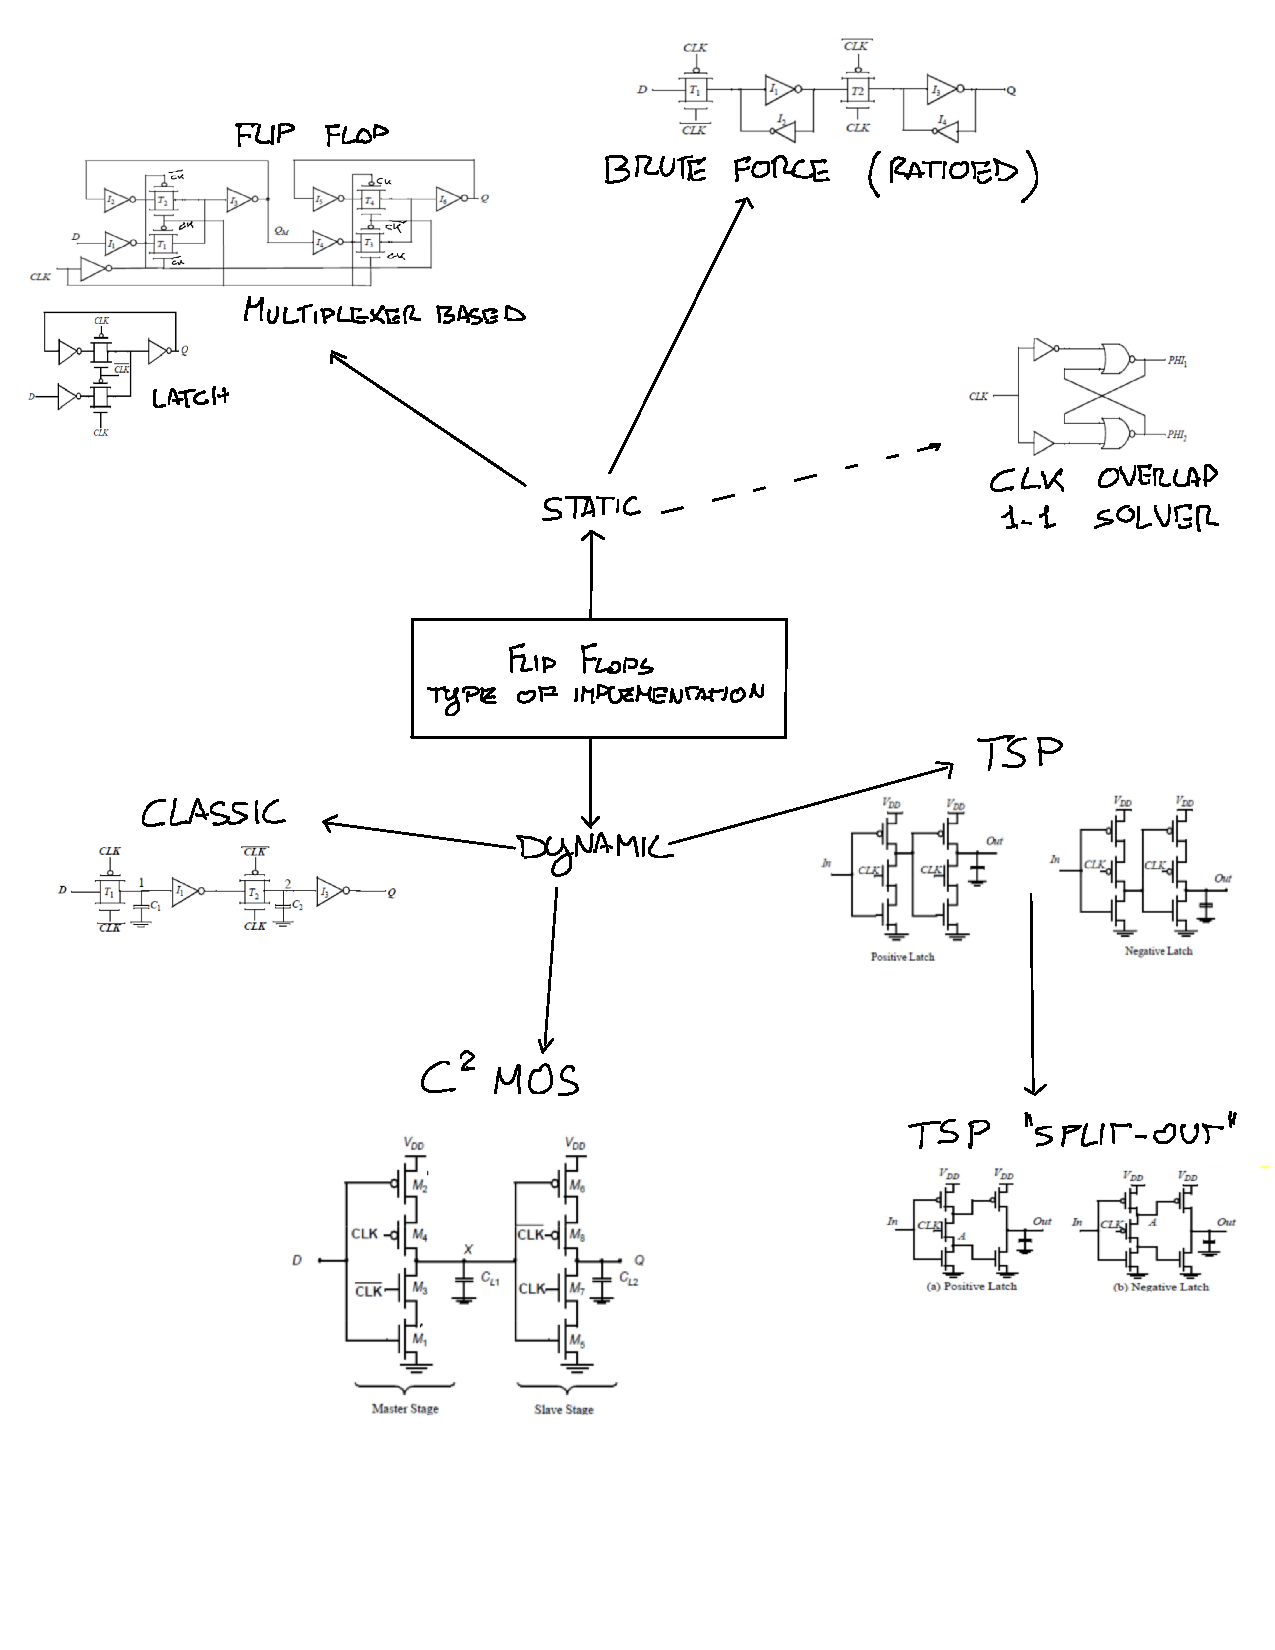
\includepdf[pages=1]{ff.pdf}

